\chapter{Empirische Evaluation}

Dieses Kapitel berichtet die Ergebnisse entlang der vier Forschungsfragen. Zunächst wird der
zusätzliche Nutzen der task-adaptiven Repräsentationsanpassung untersucht (FF1) und über
unterschiedliche Labelbudgets weiterverfolgt (FF2). FF3 prüft anschließend, ab welchem
reduzierten Labelbudget die kombinierte RUT-Repräsentation das Niveau vollständig mit
200.000 Labels trainierter Referenzen über alle fünf Evaluationsbedingungen erreicht. FF4
wechselt auf die Systemebene und untersucht die zusätzlichen Beiträge von HTML-Text, DOM
und Gating sowie die Auswirkungen der URL-first-Kaskade auf Leistung und Inferenzaufwand.
Konfidenzintervalle, p-Werte und gegebenenfalls korrigierte p-Werte werden unmittelbar bei den
jeweiligen Ergebnissen berichtet. Abschnitt 6.6 ergänzt die Auswertung um eine Unsicherheits-
und Prävalenzeinordnung der finalen Rankingmetriken.

\section{Versuchsrahmen}

Die Evaluation verwendet den in Abschnitt 4.2 definierten Data Freeze mit insgesamt
442.060 Rolleninstanzen. Davon entfallen 4.000 Instanzen auf SUP, 20.000 auf DEV, 200.000
auf den für TAPT und die nachgelagerte Labelbudgetanalyse verwendeten SSL-Pool, 50.000
ausschließlich legitime Instanzen auf CAL sowie 168.060 Instanzen auf FINAL. Die
ursprüngliche Repräsentations- und Systementwicklung wurde vor dem Zugriff auf CAL und
FINAL abgeschlossen. Die später ergänzten Labelbudget-, Komponenten- und
Sensitivitätsanalysen werden entsprechend der in Abschnitt 4.6 beschriebenen zeitlichen
Reihenfolge getrennt ausgewiesen.

Für FINAL wird die TPR bei einer auf CAL für 0,5\,\% FPR bestimmten Schwelle
berichtet. Die DEV-Auswertungen von FF1 und FF2 verwenden dagegen die interne
Teilung REP\_CAL/REP\_EVAL; die FF4-Komponentenablation nutzt ENG\_TUNE/ENG\_META. Die Schwelle wird für die FINAL-Auswertung nicht erneut
angepasst. Neben \nolinkurl{OFFICIAL_TEST} werden \nolinkurl{DOMAIN_OOD_EXACT},
\nolinkurl{TEMPLATE_OOD_EXACT}, \nolinkurl{DOMAIN_TEMPLATE_OOD_EXACT} und
\nolinkurl{LATE_TEST_Q4} ausgewertet. Die jeweiligen Umfänge betragen 168.060, 115.917,
161.223, 110.095 und 46.784 Webseiten. Die vier Teilmengen prüfen unterschiedliche
Eigenschaften der Testdaten; aus ihrer Reihenfolge wird keine Schwierigkeitsskala abgeleitet. FF1 und die ursprünglichen Lernkurven von FF2 beruhen auf fünf gepaarten Wiederholungen.
Für den zentralen Equal-Budget-Vergleich und die Labelbudgetanalyse werden fünf weitere
Wiederholungen ergänzt. N10 variiert damit Labelauswahl und Downstream-Training bei
unveränderten TAPT-Checkpoints. Die sequenzielle FF4-Komponentenablation verwendet zehn
neu festgelegte gepaarte Replikationen auf Development-Daten. Der Frontend-Vergleich der
Kaskade basiert auf fünf Systemläufen.

\section{FF1: Task-adaptive Repräsentationsanpassung}

FF1 vergleicht die vier in Abschnitt 4.3.1 definierten Repräsentationszustände R0, RT, RU
und RUT mit identischen 20.000 gelabelten Trainingsinstanzen und korrespondierenden Seeds.
R0 kombiniert dabei die allgemein selbstüberwacht vortrainierten Basisencoder. Geändert wird
ausschließlich, ob URL, HTML-Text oder beide Modalitäten zusätzlich mittels TAPT angepasst
wurden. Mit der linearen Probe steigt die mittlere TPR am festgelegten Low-FPR-Betriebspunkt von
81,35\,\% für R0 auf 87,56\,\% für RT und 88,95\,\% für RU; RUT erreicht 90,05\,\%.
Mit der MLP-Probe ergibt sich dasselbe Rangmuster mit 91,17\,\% für RUT. Die mittleren
RUT--R0-Differenzen betragen damit +8,70 beziehungsweise +8,73 Prozentpunkte. Die
faktorielle Interaktion
\[
(RUT-RT)-(RU-R0)
\]
beträgt jedoch $-5{,}10$ Prozentpunkte für die lineare Probe und $-2{,}83$ Prozentpunkte
für die MLP-Probe. Die isolierten Adaptationsgewinne von URL und HTML-Text addieren sich
damit nicht vollständig.

\begin{table}[htbp]
\centering
\caption{FF1: DEV-Ergebnisse bei 20.000 Labels, Mittelwerte über fünf Wiederholungen.}
\label{tab:ff1_dev}
\small
\begin{tabular}{llrrr}
\toprule
Probe & Rep. & TPR@0,5\,\% FPR & FPR & FPR@TPR90 \\
\midrule
Linear & R0  & 81,35\,\% & 0,53\,\% & 1,316\,\% \\
Linear & RT  & 87,56\,\% & 0,64\,\% & 0,908\,\% \\
Linear & RU  & 88,95\,\% & 0,42\,\% & 0,480\,\% \\
Linear & RUT & 90,05\,\% & 0,42\,\% & 0,408\,\% \\
\addlinespace
MLP & R0  & 82,44\,\% & 0,58\,\% & 1,360\,\% \\
MLP & RT  & 86,68\,\% & 0,63\,\% & 0,956\,\% \\
MLP & RU  & 89,76\,\% & 0,51\,\% & 0,492\,\% \\
MLP & RUT & 91,17\,\% & 0,49\,\% & 0,412\,\% \\
\bottomrule
\end{tabular}
\end{table}

Auch aus der umgekehrten Betriebspunktperspektive ergibt sich dasselbe Bild. Wird die TPR
auf mindestens 90\,\% angehoben, gibt FPR@TPR90 die False-Positive-Rate am
ersten entsprechenden ROC-Punkt an; niedrigere
Werte sind entsprechend günstiger. RUT erreicht mit 0,408\,\% beziehungsweise 0,412\,\%
die niedrigste mittlere FPR beider Probes. Die Repräsentationsauswahl wird damit durch zwei
komplementäre Low-FPR-Perspektiven gestützt. Bei fünf Beobachtungspaaren beträgt der
kleinste mögliche zweiseitige p-Wert des exakten Sign-Flip-Tests 0,0625. Die inferenzstatistische
Prüfung des zentralen RUT--R0-Vergleichs erfolgt mit zehn Beobachtungspaaren
auf FINAL in Abschnitt 6.4. Wegen der anderen Evaluationspopulation ist dies keine
inferenzstatistische Nachprüfung desselben DEV-Effekts.

\begin{figure}[!ht]
\centering
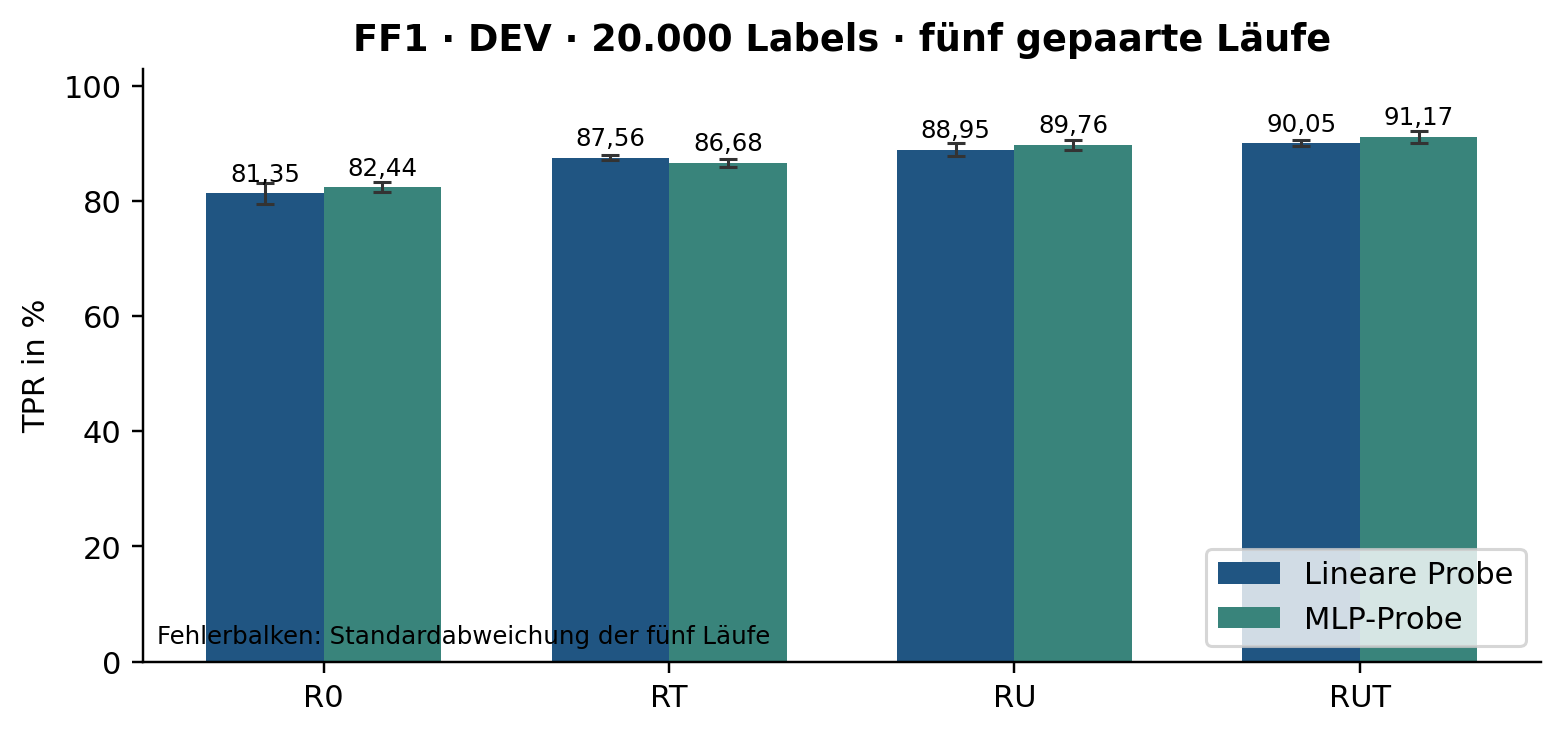
\includegraphics[width=0.82\textwidth]{Praefix/Image/06_1_FF1_ABLATION.png}
\caption{FF1: TPR der vier Repräsentationsvarianten mit linearer und MLP-Downstream-Probe.}
\label{fig:ff1_ablation}
{\footnotesize Eigene Darstellung; KI-unterstützt.}
\end{figure}

\section{FF2: Einfluss der Labelverfügbarkeit}

FF2 untersucht den Repräsentationsvergleich über sieben verschachtelte Labelbudgets von
2.000 bis 200.000 Instanzen. Die Encoder bleiben je Repräsentationszustand unverändert;
variiert wird ausschließlich die gelabelte Downstream-Supervision.

\begin{table}[H]
\centering
\caption{FF2: Mittlere FINAL-TPR der linearen Probe über die Labelbudgets.}
\label{tab:ff2_linear}
\small
\renewcommand{\arraystretch}{0.95}
\begin{tabular}{rrrrr}
\toprule
Labels & R0 & RT & RU & RUT \\
\midrule
2.000   & 51,64\% & 52,91\% & 58,62\% & 60,94\% \\
5.000   & 62,10\% & 65,07\% & 65,21\% & 67,96\% \\
10.000  & 68,00\% & 71,28\% & 71,10\% & 73,51\% \\
20.000  & 71,63\% & 75,90\% & 75,20\% & 77,73\% \\
50.000  & 75,12\% & 79,32\% & 78,97\% & 82,01\% \\
100.000 & 76,99\% & 81,04\% & 81,36\% & 84,04\% \\
200.000 & 77,92\% & 82,26\% & 83,40\% & 85,72\% \\
\bottomrule
\end{tabular}
\end{table}

Für die lineare Probe zeigt sich über das gesamte Budgetraster ein Vorteil von RUT gegenüber
R0. Die mittlere FINAL-TPR steigt für RUT von 60,94\,\% bei 2.000 Labels auf
77,73\,\% bei 20.000 und 85,72\,\% bei 200.000 Labels; R0 erreicht an denselben
Punkten 51,64\,\%, 71,63\,\% und 77,92\,\%.

Auch mit der nichtlinearen MLP-Probe bleibt dieses Rangmuster bestehen. Der Abstand zwischen
RUT und R0 beträgt bei 2.000 Labels 10,77 Prozentpunkte, bei 20.000 Labels
8,59 Prozentpunkte und bei 200.000 Labels noch 5,30 Prozentpunkte.

\begin{table}[H]
\centering
\caption{FF2: Mittlere FINAL-TPR der MLP-Probe über die Labelbudgets.}
\label{tab:ff2_mlp}
\small
\renewcommand{\arraystretch}{0.95}
\begin{tabular}{rrrrr}
\toprule
Labels & R0 & RT & RU & RUT \\
\midrule
2.000   & 42,31\% & 43,34\% & 50,30\% & 53,08\% \\
5.000   & 53,68\% & 55,44\% & 60,49\% & 63,32\% \\
10.000  & 60,94\% & 63,64\% & 67,23\% & 69,81\% \\
20.000  & 68,27\% & 72,24\% & 74,67\% & 76,86\% \\
50.000  & 78,85\% & 82,06\% & 83,63\% & 85,31\% \\
100.000 & 82,40\% & 86,33\% & 87,09\% & 89,89\% \\
200.000 & 84,95\% & 87,88\% & 88,35\% & 90,25\% \\
\bottomrule
\end{tabular}
\end{table}

Der Vorteil der task-adaptierten Repräsentation bleibt damit bei beiden
Downstream-Klassifikatoren über sämtliche untersuchten Labelbudgets bestehen. Auf DEV erreicht RUT als
ergänzende Sättigungsperspektive mit der linearen Probe 95\,\% des eigenen
200k-Niveaus bereits bei 10.000 Labels, während R0 hierfür 50.000 Labels benötigt.
Beim MLP liegen die entsprechenden B95-Punkte bei 50.000 beziehungsweise 100.000
Labels. Auf FINAL liegt B95 dagegen für R0 und RUT jeweils bei 50.000 Labels
mit der linearen Probe und bei 100.000 Labels mit dem MLP. Die frühere relative
Sättigung von RUT auf DEV überträgt sich somit nicht auf diese FINAL-Kennzahl.
Da B95 jeweils auf das eigene Endniveau einer Variante bezogen ist, wird die
absolute Performance-Suffizienz gegenüber vollständig trainierten Referenzen erst in FF3
geprüft. Zur zusätzlichen Prüfung der Label-Effizienz außerhalb des PhreshPhish-Datenbestands werden
R0 und RUT auf dem unabhängig erhobenen Phishing Website Dataset von Putra (2023)
verglichen. Auf dem zeitlich früheren Datenbestand werden identische, verschachtelte
Stichproben von 200, 500, 1.000 und 2.000 gelabelten Webseiten für zehn gepaarte
Linear-Probes verwendet und auf dem zeitlich späteren Bestand ausgewertet. Über die gesamte externe Lernkurve erreicht RUT eine mittlere AP-AULC von 91,98\,\%
gegenüber 89,45\,\% für R0. Die gepaarte Differenz beträgt +2,54 Prozentpunkte
(95\,\%-KI [2,16; 2,91], 10/10 positive Paare, $p=0{,}001953$).

\begin{table}[H]
\centering
\caption{FF2: Externe Label-Effizienz von R0 und RUT auf dem Putra-Datensatz.}
\label{tab:ff2_putra}
\small
\renewcommand{\arraystretch}{0.95}
\begin{tabular}{rrrrl}
\toprule
Labels & R0 AP & RUT AP & $\Delta$ AP & 95\,\%-KI \\
\midrule
200   & 83,91\% & 86,51\% & +2,60 pp & [1,70; 3,51] \\
500   & 88,96\% & 91,76\% & +2,79 pp & [2,22; 3,36] \\
1.000 & 91,70\% & 94,05\% & +2,35 pp & [2,02; 2,69] \\
2.000 & 93,40\% & 95,61\% & +2,21 pp & [1,85; 2,56] \\
\bottomrule
\end{tabular}
\end{table}

Die zusätzliche Zielanpassung von Quell-RUT auf dem frühen Putra-Pool verbessert
dieses Ergebnis nicht. Ihre mittlere AP-AULC fällt von 91,98\,\% auf 90,84\,\%;
die gepaarte Differenz beträgt $-1{,}14$ Prozentpunkte
(95-\%-KI [$-1{,}50$; $-0{,}78$], zehn negative Paare, $p=0{,}001953125$).
Die budgetweisen AP-Differenzen betragen bei 200, 500, 1.000 und 2.000 Labels
$-2{,}28$, $-1{,}31$, $-0{,}49$ und $-0{,}51$ Prozentpunkte.
Auch diese vier Unterschiede bleiben nach Holm-Korrektur signifikant
($p_{\mathrm{Holm}}\leq0{,}01171875$). Der Vorteil von Quell-RUT gegenüber R0
und die Verschlechterung durch eine weitere Zielanpassung betreffen verschiedene
Interventionen; der zweite Befund begrenzt eine pauschale Empfehlung wiederholten TAPT.

RUT erreicht damit an allen vier externen Labelbudgets eine höhere mittlere AP.
Sämtliche budgetweisen Vergleiche bleiben nach Holm-Korrektur signifikant
($p_{\mathrm{Holm}}=0{,}007812$). Der innerhalb von PhreshPhish beobachtete Vorteil
der task-adaptierten Repräsentation bleibt somit auch unter begrenzter gelabelter
Supervision auf dem unabhängig erhobenen Webseitenbestand bestehen. Abbildung~\ref{fig:ff2_curves} fasst abschließend die internen Lernkurven der vier
Repräsentationsvarianten zusammen. Die externe Putra-Auswertung wird aufgrund des
abweichenden Budgetrasters separat in Tabelle~\ref{tab:ff2_putra} ausgewiesen.

\begin{figure}[H]
\centering
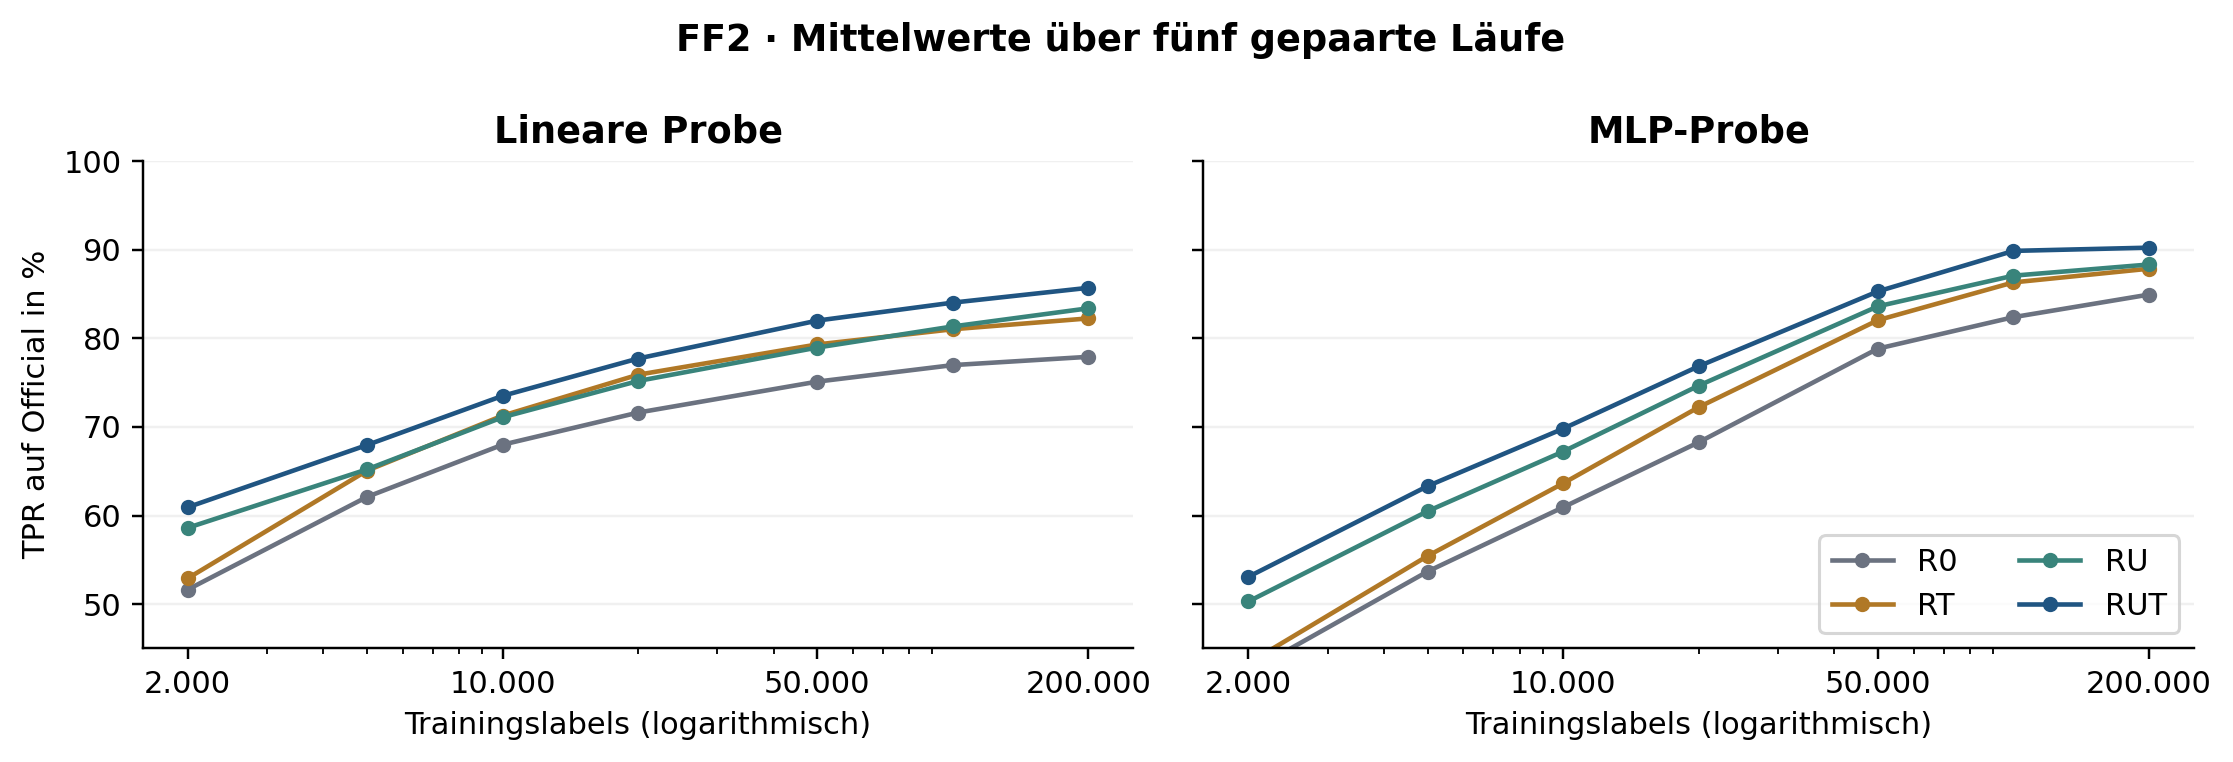
\includegraphics[width=0.78\textwidth]{Praefix/Image/06_2_FF2_LEARNING_CURVES.png}
\caption{FF2: Lernkurven der Repräsentationsvarianten über die sieben Labelbudgets mit
linearer und MLP-Probe.}
\label{fig:ff2_curves}
{\footnotesize Eigene Darstellung; KI-unterstützt.}
\end{figure}

\section{FF3: Erreichen des 200k-Referenzniveaus}

FF3 verbindet die Labelkurven mit den fünf Evaluationsbedingungen. Zunächst wird der zentrale
Vergleich zwischen RUT und R0 bei 20.000 Labels auf zehn gepaarte Wiederholungen erweitert.
Auf \nolinkurl{OFFICIAL_TEST} erreicht RUT eine TPR von 77,51\,\% gegenüber 71,43\,\% für
R0. Die mittlere gepaarte Differenz beträgt damit +6,08 Prozentpunkte
(95-\%-KI [5,38; 6,79]); alle zehn Paare zeigen einen positiven Unterschied
($p=0{,}001953$).

Auch auf Domain-OOD, Template-OOD, Domain+Template-OOD und Late Q4 liegt RUT über
R0. Die mittleren Unterschiede betragen +5,64, +6,26, +5,89 und +5,51 Prozentpunkte.
Die vier p-Werte bleiben nach Holm-Korrektur signifikant
($p_{\mathrm{Holm}}=0{,}007812$). Gleichzeitig ist die mittlere FPR von RUT in allen fünf
Bedingungen niedriger als diejenige von R0.

Anschließend wird RUT über das vollständige Budgetraster mit zwei Referenzen verglichen, die
jeweils mit 200.000 Labels trainiert wurden. Gegen R0@200k bleiben Repräsentationsformat und
Linear Probe identisch. Ein RUT-Budget wird nur dann als ausreichend bewertet, wenn die
festgelegte Nichtunterlegenheitsbedingung von einem Prozentpunkt in allen fünf
Evaluationsbedingungen erfüllt wird und die anschließende Holm-Korrektur über die sieben
Budgetentscheidungen bestehen bleibt. Abbildung~\ref{fig:ff3_heatmap} zeigt die absoluten mittleren TPR-Werte der
RUT-Repräsentation über die fünf Evaluationsbedingungen und ausgewählte Trainingsbudgets.
Die Werte steigen in allen Bedingungen mit wachsendem Labelbudget. Die Darstellung allein
legt jedoch noch keine ausreichende Budgetstufe fest; hierfür ist der statistische Vergleich mit
den beiden 200k-Referenzen maßgeblich.

\begin{figure}[!ht]
\centering
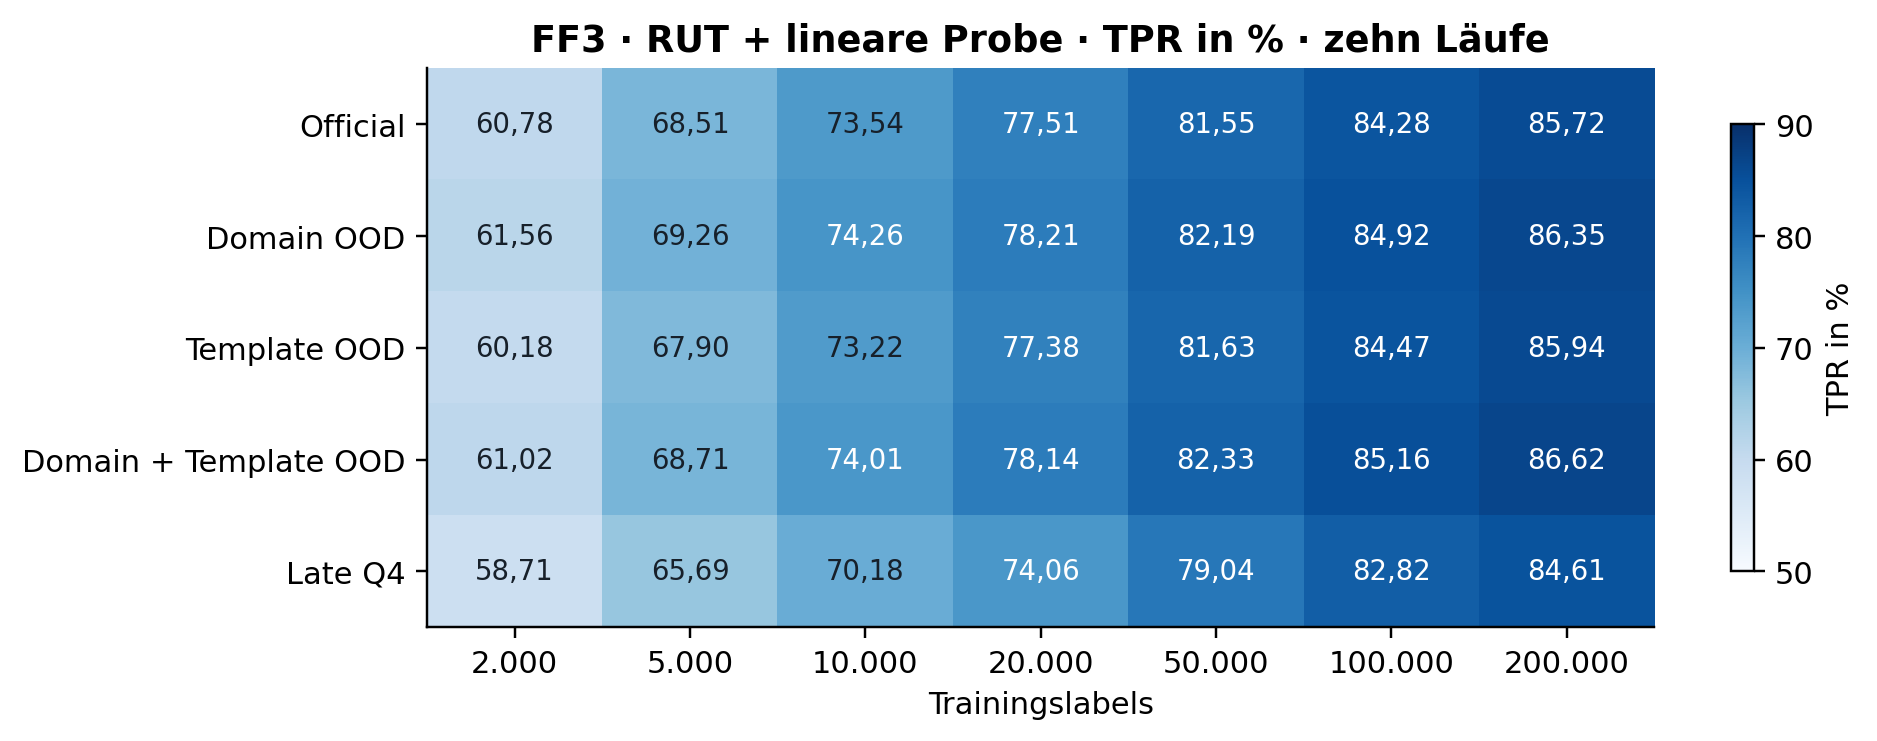
\includegraphics[width=0.76\textwidth]{Praefix/Image/FF3_RUT_TPR_Heatmap.png}
\caption{FF3: Mittlere RUT-TPR über fünf Evaluationsbedingungen und ausgewählte Labelbudgets, N10-Mittelwerte.}
\label{fig:ff3_heatmap}
{\footnotesize Eigene Darstellung; KI-unterstützt.}
\end{figure}

Gegen R0@200k reichen 20.000 Labels nach dieser Entscheidungsregel noch nicht aus. Der
ungünstigste mittlere TPR-Abstand tritt auf Late Q4 auf und beträgt $-1{,}37$
Prozentpunkte. Mit 50.000 Labels wird die Nichtunterlegenheitsbedingung dagegen in allen fünf
Bedingungen erfüllt; die korrigierte Entscheidung bleibt nach Holm signifikant
($p_{\mathrm{Holm}}=0{,}006836$). Die mittlere TPR von RUT50k liegt dabei in allen fünf
Bedingungen um +3,24 bis +3,62 Prozentpunkte über R0@200k. Gleichzeitig fällt die mittlere
realisierte FPR um 0,079 bis 0,180 Prozentpunkte niedriger aus. Als zweite Referenz dient die unabhängig trainierte TF-IDF/XGBoost-Pipeline mit 200.000
Labels. Tabelle~\ref{tab:ff3_xgb} zeigt die Ergebnisse für die beiden RUT-Budgets von 20.000
und 50.000 Labels. Bereits RUT20k erreicht in allen fünf Bedingungen mindestens die mittlere
XGBoost-TPR und zugleich eine niedrigere mittlere FPR. Der kleinste TPR-Vorsprung beträgt
auf Late Q4 allerdings nur +0,09 Prozentpunkte.

Die fünf einzelnen Nichtunterlegenheitstests für RUT20k erfüllen jeweils die
1-pp-Bedingung, die gemeinsame Budgetentscheidung erreicht nach der Holm-Korrektur über
alle sieben getesteten Budgets jedoch nicht das festgelegte Signifikanzniveau
($p_{\mathrm{Holm}}=0{,}173233$). RUT20k übertrifft XGBoost@200k damit deskriptiv in allen
fünf betrachteten Bedingungen, reicht für die strengere statistische Budgetentscheidung jedoch
nicht aus.

\begin{table}[htbp]
\centering
\caption{FF3: RUT bei 20k und 50k Labels gegenüber TF-IDF/XGBoost@200k, N10-Mittelwerte.}
\label{tab:ff3_xgb}
\small
\begin{tabular}{lrrrrrr}
\toprule
 & \multicolumn{2}{c}{XGB@200k} & \multicolumn{2}{c}{RUT20k} & \multicolumn{2}{c}{RUT50k} \\
Bedingung & TPR & FPR & TPR & FPR & TPR & FPR \\
\midrule
Official & 76,96\,\% & 0,618\,\% & 77,51\,\% & 0,520\,\% & 81,55\,\% & 0,537\,\% \\
Domain-OOD & 76,98\,\% & 1,219\,\% & 78,21\,\% & 0,951\,\% & 82,19\,\% & 0,979\,\% \\
Template-OOD & 76,75\,\% & 0,604\,\% & 77,38\,\% & 0,516\,\% & 81,63\,\% & 0,533\,\% \\
Domain+Template & 76,75\,\% & 1,186\,\% & 78,14\,\% & 0,938\,\% & 82,33\,\% & 0,966\,\% \\
Late Q4 & 73,97\,\% & 1,127\,\% & 74,06\,\% & 0,681\,\% & 79,04\,\% & 0,728\,\% \\
\bottomrule
\end{tabular}
\end{table}

Mit 50.000 Labels wird die Nichtunterlegenheitsbedingung gegenüber XGBoost@200k in allen
fünf Bedingungen erfüllt. Der gemeinsame p-Wert beträgt $2{,}561\times10^{-6}$ und nach
Holm-Korrektur $1{,}281\times10^{-5}$. Die mittlere TPR von RUT50k liegt je nach Bedingung
um +4,59 bis +5,58 Prozentpunkte höher, während gleichzeitig eine um 0,071 bis
0,398 Prozentpunkte niedrigere FPR erreicht wird.

50.000 Labels sind damit die kleinste untersuchte RUT-Stufe, die die festgelegte
Nichtunterlegenheitsbedingung sowohl gegenüber R0@200k als auch gegenüber
TF-IDF/XGBoost@200k über alle fünf Evaluationsbedingungen erfüllt. Gegenüber einem
Labelbudget von 200.000 Instanzen entspricht dies einer Reduktion der gelabelten
Downstream-Trainingsmenge um 75\,\%. Der vorausgehende TAPT-Schritt auf 200.000
ungelabelten Webseiten bleibt davon unberührt.

Die ergänzende Sensitivitätsanalyse mit TPR-Margen von 0,0, 0,5, 1,0 und 2,0
Prozentpunkten bestätigt die Stabilität dieser Budgetentscheidung. In allen vier Fällen bleiben
50.000 Labels die kleinste RUT-Stufe, die die jeweilige Testentscheidung gegenüber beiden
200k-Referenzen erfüllt. Auch ohne zugelassenen TPR-Nachteil ($\Delta=0{,}0$ pp) bleibt
RUT50k gegenüber R0@200k ($p_{\mathrm{Holm}}=0{,}006836$) und
TF-IDF/XGBoost@200k ($p_{\mathrm{Holm}}=6{,}286\times10^{-5}$) statistisch gestützt.
RUT20k reicht gegenüber R0@200k selbst bei einer auf 2,0 Prozentpunkte erweiterten Marge
nicht aus ($p_{\mathrm{Holm}}=0{,}593750$); gegenüber XGBoost@200k wird 20k erst bei
dieser 2-pp-Marge statistisch gestützt ($p_{\mathrm{Holm}}=0{,}008464$). Die gemeinsame
50k-Entscheidung bleibt damit über den untersuchten Margenbereich von 0 bis 2
Prozentpunkten unverändert.

Abbildung~\ref{fig:ff3_cross} stellt für beide Referenzen jeweils den ungünstigsten mittleren
TPR-Abstand über die fünf Evaluationsbedingungen dar. Bei 20.000 Labels liegt RUT gegenüber
XGBoost bereits knapp oberhalb der Null-Linie, gegenüber R0@200k jedoch noch unter der
festgelegten Marge. Ab 50.000 Labels sind die mittleren Abstände zu beiden Referenzen in allen
Bedingungen positiv.

\begin{figure}[!ht]
\centering
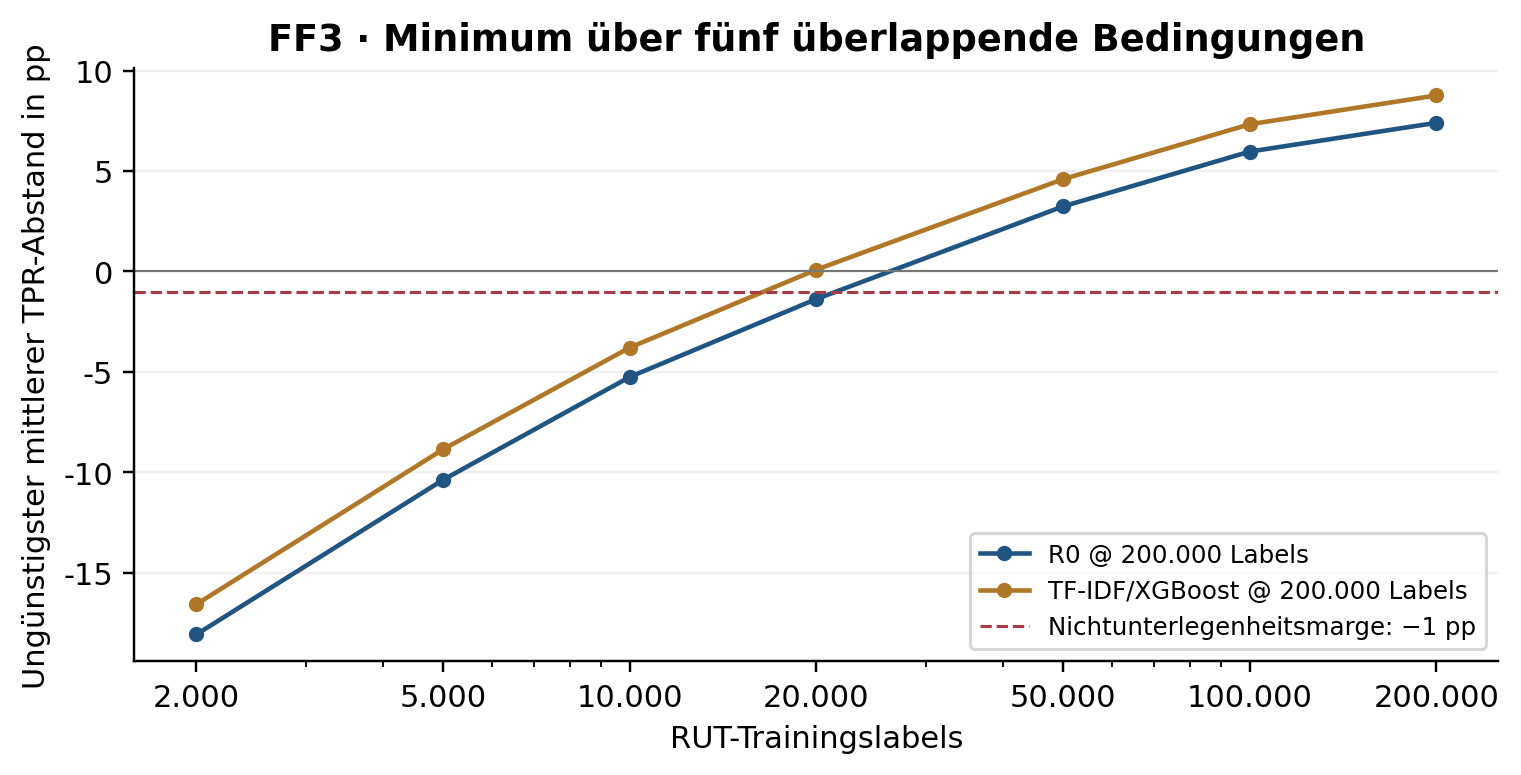
\includegraphics[width=0.80\textwidth]{Praefix/Image/FF3_Worst_Case_Gaps.png}
\caption{FF3: Schlechtester mittlerer TPR-Abstand von RUT gegenüber R0@200k und TF-IDF/XGBoost@200k über die fünf Evaluationsbedingungen.}
\label{fig:ff3_cross}
{\footnotesize Eigene Darstellung; KI-unterstützt.}
\end{figure}

\section{FF4: Inkrementeller Systembeitrag und URL-first-Verarbeitung}

FF4 untersucht den zusätzlichen Beitrag der einzelnen Systembestandteile. Hierfür wird RUT
als gemeinsame Repräsentationsbasis verwendet und auf getrennten Development-Daten eine
Folge von vier Varianten verglichen: URL-only (P0), URL+Text mit gleichgewichteter Fusion
(P1), URL+Text+DOM mit gleichgewichteter Fusion (P2) und dieselben drei Modalitäten mit
lernbarem Gating (P3). Alle Varianten erhalten innerhalb einer Replikation dieselben
20.000 Labels und werden über zehn gepaarte Wiederholungen verglichen. CAL und FINAL
werden für diese Analyse nicht verwendet.

Die mittlere TPR steigt entlang dieser Varianten von 87,932\,\% auf 93,116\,\%, 93,844\,\%
und schließlich 94,420\,\%. Den größten zusätzlichen Beitrag liefert der HTML-Text:
$P_1-P_0$ beträgt +5,184 Prozentpunkte (95-\%-KI [4,324; 6,044], 10/10 positive Paare).
Durch den DOM-Zweig steigt die TPR um weitere +0,728 Prozentpunkte
(95-\%-KI [0,305; 1,151], 10/10 positive Paare). Der Übergang von gleichgewichteter zu
lernbarer Gating-Fusion erhöht sie um weitere +0,576 Prozentpunkte
(95-\%-KI [0,226; 0,926], 9/10 positive Paare). Alle drei Vergleiche bleiben nach der
gemeinsamen Holm-Korrektur signifikant
($p_{\mathrm{Holm}}=0{,}00585938$). Die realisierte \nolinkurl{ENG_META}-FPR steigt entlang
der Varianten leicht von 0,400\,\% auf 0,616\,\%; gleichzeitig sinkt FPR@TPR90 von
0,528\,\% auf 0,260\,\%.

Die Komponentenablation wurde nach Festlegung der finalen Architektur ergänzend durchgeführt
und diente nicht zu deren nachträglicher Auswahl. Sie zeigt jedoch, dass jeder der drei
hinzugefügten Bestandteile im festgelegten Vergleich einen positiven zusätzlichen Beitrag leistet.
Passend dazu erreicht die bereits eingefrorene Gated-TRI-Konfiguration auch auf FINAL in allen
fünf Bedingungen eine höhere TPR als die gleichgewichtete Fusion. Auf
\nolinkurl{OFFICIAL_TEST} steigt die TPR von 95,65\,\% auf 96,12\,\%; in den vier
zusätzlichen Bedingungen beträgt der Unterschied 0,38 bis 0,54 Prozentpunkte. Für die Systemperspektive wird anschließend das eingefrorene TRI-Vollsystem mit der bereits vor
dem FINAL-Zugriff festgelegten URL-first-Kaskade verglichen. Auf \nolinkurl{OFFICIAL_TEST}
erreicht TRI Full 96,12\,\% TPR bei 0,666\,\% FPR, die Kaskade 95,77\,\% TPR bei
0,680\,\% FPR. Die eingefrorene Routingkonfiguration eskaliert 14,93\,\% der Webseiten;
für 85,07\,\% wird die Entscheidung bereits nach der URL-Stufe abgeschlossen. Im
In-Memory-Benchmark sinkt die Median-Latenz von 30,18 auf 11,95 ms und der Durchsatz
steigt von 183,2 auf 447,0 Seiten/s, entsprechend dem 2,44-Fachen.

\begin{table}[htbp]
\centering
\caption{FF4: In-Memory-Benchmark des vollständigen Systems und der eingefrorenen URL-first-Kaskade.}
\label{tab:ff4_runtime}
\small
\begin{tabular}{lrr}
\toprule
Kennzahl & TRI Full & TRI-Kaskade \\
\midrule
TPR, Official & 96,12\,\% & 95,77\,\% \\
FPR, Official & 0,666\,\% & 0,680\,\% \\
Eskalation, Official & 100,00\,\% & 14,93\,\% \\
\addlinespace
Median-Latenz, DEV, Batch 1 & 30,18 ms & 11,95 ms \\
95. Perzentil, DEV, Batch 1 & 47,40 ms & 32,14 ms \\
Durchsatz, DEV, Batch 32 & 183,18 Seiten/s & 447,02 Seiten/s \\
Durchsatz-Standardabweichung, drei Läufe & 1,32 Seiten/s & 2,95 Seiten/s \\
Peak-VRAM, DEV, Batch 1 & 1.022,32 MiB & 966,77 MiB \\
Peak-VRAM, DEV, Batch 32 & 1.199,81 MiB & 1.051,72 MiB \\
\bottomrule
\end{tabular}
\end{table}

Der ergänzende Frontend-Vergleich untersucht anschließend eine andere Frage. TRI-Fallback
und Routinglogik bleiben gleich; lediglich die URL-Repräsentation wird zwischen
\nolinkurl{URL_BASE} und \nolinkurl{URL_TAPT} variiert. Für beide Varianten werden auf
Development dieselben zulässigen TPR-Abweichungen gegenüber dem Vollsystem verwendet.
Diese Analyse ist von der zuvor eingefrorenen Kaskadenkonfiguration mit einer Eskalationsrate
von 14,93\,\% zu unterscheiden; die absoluten Eskalationsraten beider Versuchsblöcke sind
deshalb nicht direkt miteinander vergleichbar.

Abbildung~\ref{fig:ff4_combined} fasst die beiden für FF4 zentralen Architektur- und
Ressourcenbefunde zusammen. Panel~(a) zeigt die sequenzielle Komponentenablation, Panel~(b)
die mittlere Eskalationsrate auf dem vollständigen Official-Testbestand über die
vier untersuchten TPR-Toleranzen.

\begin{figure}[!ht]
\centering
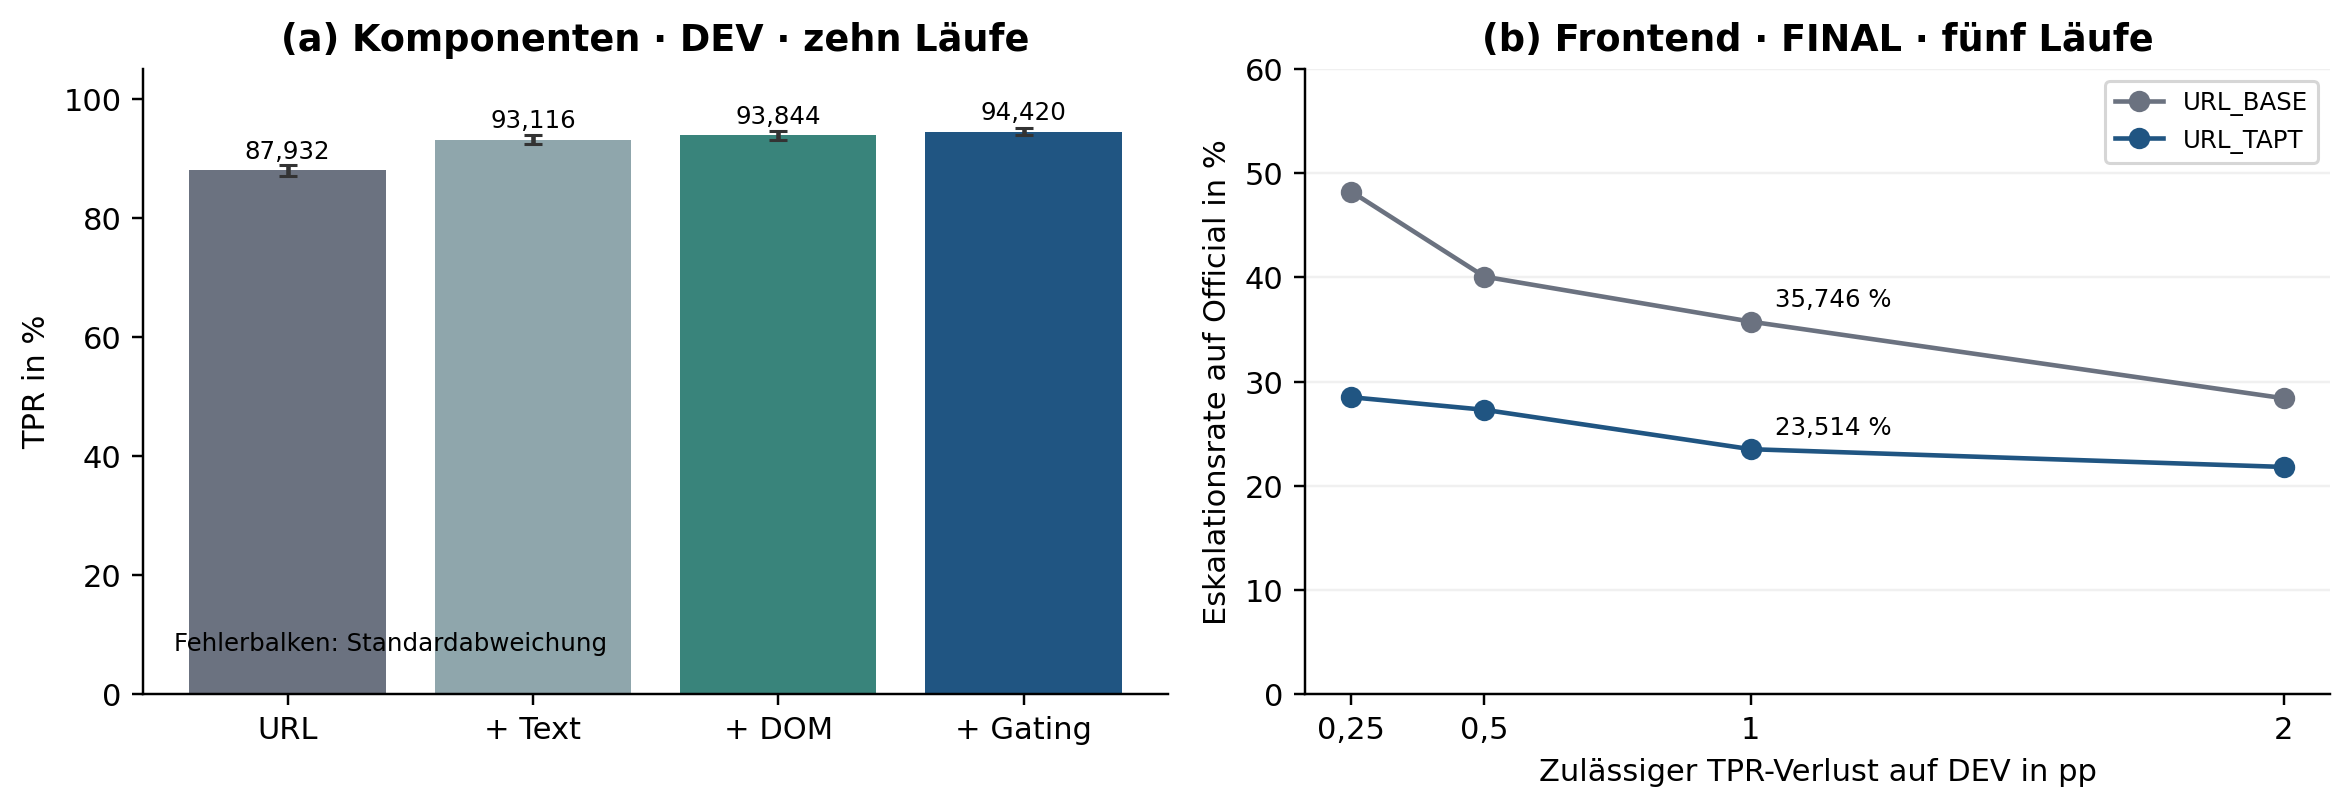
\includegraphics[width=0.90\textwidth]{Praefix/Image/FF4_Komponentenablation_Frontendvergleich.png}
\caption{FF4: Sequenzielle Komponentenablation und URL-first-Frontendvergleich von \nolinkurl{URL_BASE} und \nolinkurl{URL_TAPT}.}
\label{fig:ff4_combined}
{\footnotesize Eigene Darstellung; KI-unterstützt.}
\end{figure}

Bei der primären Toleranz von einem Prozentpunkt sinkt der ungewichtete
Szenariomittelwert der Eskalationsrate mit dem task-adaptierten URL-Frontend
von 41,125\,\% auf 28,728\,\%. Die fünf Szenarien überlappen; dieser Makromittelwert
beschreibt deshalb keine disjunkte Gesamtpopulation. Der Unterschied beträgt
12,397 Prozentpunkte. Der entsprechende Makromittelwert des Anteils früher URL-Entscheidungen beträgt
71,272\,\%. Die niedrigere Eskalationsrate von \nolinkurl{URL_TAPT} zeigt sich
in allen fünf Evaluationsbedingungen und liegt dort zwischen 10,810 und 13,438 Prozentpunkten
unter \nolinkurl{URL_BASE}. Die mittlere TPR-Abweichung vom Vollsystem beträgt
$-0{,}791$ Prozentpunkte, die mittlere FPR-Differenz $-0{,}014$ Prozentpunkte. Unter
derselben auf Development festgelegten TPR-Toleranz benötigt das task-adaptierte
URL-Frontend damit seltener die nachgelagerte vollständige multimodale Verarbeitung.

Auf dem vollständigen \nolinkurl{OFFICIAL_TEST} beträgt die mittlere Eskalationsrate
35,746\,\% für URL\_BASE und 23,514\,\% für URL\_TAPT
(Differenz $-12{,}232$ Prozentpunkte, fünf Läufe). URL\_TAPT schließt dort
76,486\,\% der Webseiten im URL-Pfad ab. Gegenüber dem Vollsystem beträgt die
TPR-Differenz $-0{,}940$ und die FPR-Differenz $+0{,}016$ Prozentpunkte.
Die niedrigere Eskalation geht somit mit einem kleinen Qualitätsverlust gegenüber
dem Vollsystem einher; die auf DEV gewählte Toleranz garantiert keine identische Test-TPR.

\section{Ergänzende Unsicherheits- und Prävalenzeinordnung}

Ergänzend zur Betriebspunktanalyse werden AP und $P_{\geq 90}$ auf dem festen
\nolinkurl{OFFICIAL_TEST} mit 1.000 stratifizierten Bootstrap-Replikationen ausgewertet.
TRI Full erreicht eine AP von 99,679\,\% mit einem 95-\%-Percentile-Intervall von
[99,659; 99,700]\,\% sowie ein $P_{\geq 90}$ von 99,714\,\%
[99,673; 99,753]\,\%. Die Kaskade erreicht eine AP von 98,539\,\%
[98,476; 98,602]\,\% und ein $P_{\geq 90}$ von 99,776\,\%
[99,742; 99,815]\,\%. Die engen Intervalle zeigen eine geringe Stichprobenunsicherheit
dieser Rankingmetriken auf dem festen Testbestand. Für die absolute Höhe precision-basierter Kennzahlen ist zusätzlich die Klassenprävalenz
relevant, also der Anteil phishingbezogener Webseiten innerhalb der Evaluationsmenge. Der
\nolinkurl{OFFICIAL_TEST} enthält 76.800 Phishing- und 91.260 Benign-Instanzen und weist
damit einen Phishing-Anteil von 45,70\,\% auf. Dies entspricht nahezu der für den regulären
PhreshPhish-Testbestand berichteten Base Rate von 46\,\%
(vgl. [Dalton et al. (2026), S. 6--7]). Zur Einordnung wird deshalb eine reine
Base-Rate-Sensitivität von $P_{\geq 90}$ berechnet. Für die ausgewählte Schwelle
werden die klassenspezifischen Scoreverteilungen konstant gehalten und ausschließlich
die angenommene Prävalenz verändert. Mit der beobachteten Precision $P_0$ und
der Testprävalenz $\pi_0=76.800/168.060$ gilt
\[
\lambda=\frac{1-P_0}{P_0}\frac{\pi_0}{1-\pi_0}
       =\frac{\mathrm{FPR}_*}{\mathrm{TPR}_*},
\qquad
\mathrm{Precision}_{\pi}=\frac{\pi}{\pi+(1-\pi)\lambda}.
\]
Hierbei kennzeichnet $*$ die für $P_{\geq 90}$ ausgewählte empirische Schwelle.
Die Umrechnung benötigt keinen Recall von exakt 90\,\%. Sie bildet einen reinen
Prior-Shift ab; Veränderungen des klassenspezifischen Fehlerverhaltens sind darin
nicht enthalten.

\begin{table}[htbp]
\centering
\caption{Base-Rate-Sensitivität von $P_{\geq 90}$.}
\label{tab:base_rate_sensitivity}
\small
\begin{tabular}{lrr}
\toprule
Phishing-Base-Rate & TRI Full & TRI-Kaskade \\
\midrule
45,70\,\% & 99,714\,\% & 99,776\,\% \\
5\,\%     & 95,62\,\%  & 96,54\,\% \\
1\,\%     & 80,74\,\%  & 84,27\,\% \\
\bottomrule
\end{tabular}
\end{table}

Die rechnerischen Werte bei 1\,\% Base Rate betragen 80,74\,\% für TRI Full und
84,27\,\% für die Kaskade. Sie sind keine Messungen auf einem neu erhobenen Bestand
mit dieser Prävalenz. Ein direkter Vergleich mit separat konstruierten
PhreshPhish-Benchmarks wäre wegen unterschiedlicher Testzusammensetzung und nicht
abgeglichener Metrikimplementierung nicht belastbar. Die primäre Systembewertung
stützt sich weiterhin auf TPR und FPR am festgelegten Betriebspunkt.
